% =====================================================================
% THIS FILE IS THE SOURCE. Edit it, then rebuild the PDF with:
%     bash tools/compile.sh Unit_06_Inference_Without_a_Formula
%
% Figures are the fig_u6_*.pdf files in this folder, from
% tools/make_unit06_slide_figs.py. They run on data/rent.csv, the listings
% the Unit 5 homework used, plus one added column of pure noise.
% =====================================================================
\documentclass[aspectratio=169]{beamer}
\usetheme{default}
\usefonttheme{professionalfonts}
\usepackage{amsmath, amssymb, amsfonts}
\usepackage{graphicx}
\usepackage{booktabs}
\renewcommand{\arraystretch}{1.2}
\usepackage{array}
\newcolumntype{L}[1]{>{\raggedright\arraybackslash}p{#1}}
\usepackage{bm}
\usepackage{hyperref}

\mode<presentation> {
    \usetheme{Frankfurt}
    \usecolortheme{default}
}

\newcommand{\xbar}{\bar{x}}
\newcommand{\SE}{\mathrm{SE}}
\newcommand{\se}{\widehat{\SE}}

\newenvironment{principle}[1]{\begin{block}{\textbf{Principle:} #1}}{\end{block}}
\newenvironment{trap}[1]{\begin{alertblock}{\textbf{Trap:} #1}}{\end{alertblock}}
\newenvironment{practice}[1]{\begin{exampleblock}{\textbf{In practice:} #1}}{\end{exampleblock}}
\newenvironment{interview}[1]{\begin{exampleblock}{\textbf{You may be asked:} #1}}{\end{exampleblock}}
\newenvironment{yourturn}[1]{%
  \setbeamercolor{block title}{fg=white,bg=orange!80!black}%
  \setbeamercolor{block body}{bg=orange!12}%
  \begin{block}{\textbf{Your turn:} #1}}{\end{block}}
\newenvironment{quickcheck}[1]{%
  \setbeamercolor{block title}{fg=white,bg=teal!80!black}%
  \setbeamercolor{block body}{bg=teal!10}%
  \begin{block}{\textbf{Quick check:} #1}}{\end{block}}
\newenvironment{llmcheck}[1]{%
  \setbeamercolor{block title}{fg=white,bg=violet!75!black}%
  \setbeamercolor{block body}{bg=violet!10}%
  \begin{block}{\textbf{LLM check:} #1}}{\end{block}}

\title{Inference Without a Formula}

\begin{document}

\begin{frame}
  \titlepage
\end{frame}

% ======================================================================
\section{Why}
% ======================================================================
\begin{frame}{Where we left off}
\begin{itemize}
  \item Unit 5 ended with a tree finding a threshold, and a regression turning that threshold into
        a number with an interval on it.
  \item The regression did the reporting because the tree could not. It has no coefficients and no
        standard errors, so there was nothing to report.
  \item That was a workaround. This unit is about getting those answers out of the tree itself.
\end{itemize}
\end{frame}

\begin{frame}{What this unit gives you}
\begin{columns}[T]
\begin{column}{0.5\textwidth}
\textbf{Things to know}
\begin{itemize}\small
  \item what a variable importance score measures, and what it does not
  \item why the default importance in most software flatters some columns
  \item what permutation importance does instead
  \item how resampling your own data produces an interval
  \item how to put an interval on a quantity with no formula
  \item what resampling cannot repair
\end{itemize}
\end{column}
\begin{column}{0.5\textwidth}
\textbf{Mistakes to stop making}
\begin{itemize}\small
  \item reading an importance ranking as a ranking of effects
  \item trusting the default importance on a column with many distinct values
  \item quoting a single number for anything resampling could have given an interval for
  \item resampling before splitting the data, so the same row lands on both sides
  \item treating a bootstrap interval as a repair for a biased sample
\end{itemize}
\end{column}
\end{columns}
\end{frame}

\begin{frame}{What a model without a likelihood cannot hand you}
Unit 2 drew the line between a model that states a distribution for the outcome and one that does
not. Everything on the right of that line costs something:
\begin{center}\small
\begin{tabular}{L{0.40\textwidth} L{0.50\textwidth}}
\toprule
\textbf{From a regression} & \textbf{From a forest} \\
\midrule
a coefficient, in units & nothing directly comparable \\
a standard error & nothing \\
a confidence interval & nothing \\
a p-value & nothing \\
AIC & nothing, there is no likelihood \\
\bottomrule
\end{tabular}
\end{center}
\vspace{0.2em}
\begin{principle}{what this unit is for}
None of those gaps is permanent. Resampling rebuilds the middle three, and an importance score
covers part of the first. What they cost is compute time rather than a new assumption.
\end{principle}
\end{frame}

\begin{frame}{The data for this unit}
\texttt{rent.csv}, the 4,743 rental listings from the Unit 5 homework. Same data, a different
question: not how much a square foot is worth, but which columns the model leans on and how sure
we are of any of it.
\begin{center}\small
\begin{tabular}{L{0.26\textwidth} L{0.62\textwidth}}
\toprule
\textbf{Column} & \textbf{What it is} \\
\midrule
\texttt{Rent} & monthly rent in rupees, the outcome \\
\texttt{Size} & floor area in square feet \\
\texttt{BHK}, \texttt{Bathroom} & bedrooms, bathrooms \\
\texttt{City} & six cities \\
\texttt{FurnishingStatus} & furnished, semi, unfurnished \\
\texttt{id\_number} & \textbf{added here}: a random six-digit number, meaning nothing \\
\bottomrule
\end{tabular}
\end{center}
\vspace{0.2em}
That last column is the test. A column that cannot possibly matter tells you which importance
methods can be believed.
\end{frame}

% ======================================================================
\section{Importance}
% ======================================================================
\begin{frame}{What an importance score is}
\begin{itemize}
  \item A forest has no coefficient for \texttt{Size}, so there is no sentence of the form
        ``a square foot is worth this much''.
  \item What it can report is how much the column contributed to the fitting. That is a
        \textbf{variable importance} score.
  \item It is one number per column, always positive or near zero, with no units and no direction.
        It cannot tell you whether rent goes up or down with size.
\end{itemize}
\begin{trap}{the word does a lot of work}
Important is not the same as large, and not the same as causal. An importance score ranks columns
by how much this particular fitted model used them.
\end{trap}
\end{frame}

\begin{frame}{The default: how much splitting a column did}
\begin{itemize}
  \item Every split in every tree improves the fit by some amount. Add up those improvements for
        each column and you have \textbf{impurity importance}, which is what
        \texttt{.feature\_importances\_} returns.
  \item It is free, because the forest already did the arithmetic while it was being built.
  \item It also has a known flaw: a column with many distinct values gets many candidate cut
        points, so it wins splits by having more chances, not by carrying more signal.
\end{itemize}
\end{frame}

\begin{frame}{How to catch it}
\begin{itemize}
  \item Add a column of random six-digit numbers to the listings. It has nothing to do with rent.
        We know this, because we generated it.
  \item Fit the forest on everything, including the random column.
  \item If an importance method is trustworthy, that column should come out at the bottom.
\end{itemize}
\begin{practice}{a sanity check you can always run}
A column you know to be noise, added on purpose, is the cheapest audit of any importance method,
any feature selection routine, and any claim that a model found something.
\end{practice}
\end{frame}

\begin{frame}{Two methods, two different answers}
\centering
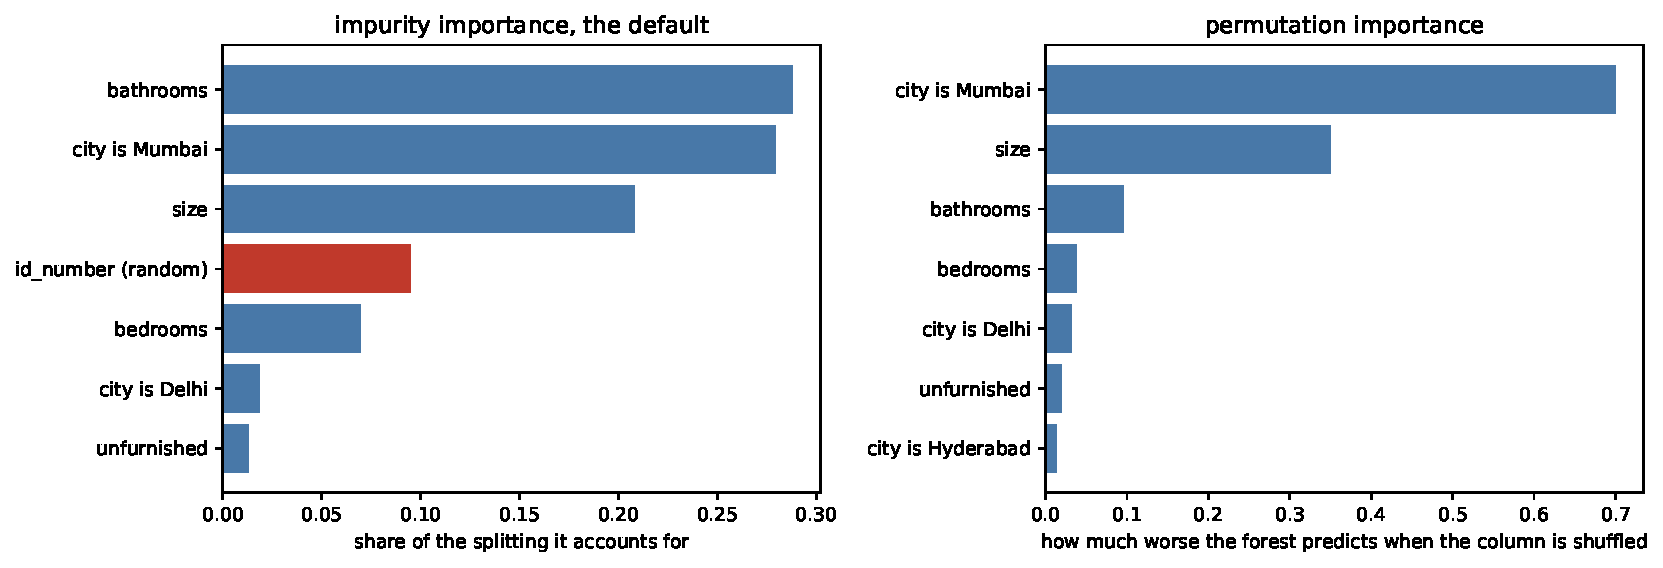
\includegraphics[width=\textwidth]{fig_u6_two_importances.pdf}
\vspace{0.2em}
\begin{minipage}{0.95\textwidth}\small
On the left, the random column places \textbf{fourth of eleven}, above bedrooms. On the right it
does not reach the top seven. The two methods also disagree about the real columns: the left
ranks bathrooms first, the right ranks Mumbai first by a wide margin.
\end{minipage}
\end{frame}

\begin{frame}{The same five columns, ranked both ways}
\begin{center}\small
\begin{tabular}{lcc}
\toprule
\textbf{Column} & \textbf{impurity} & \textbf{permutation} \\
\midrule
bathrooms & 0.288 \quad(1st) & 0.096 \quad(3rd) \\
city is Mumbai & 0.279 \quad(2nd) & 0.699 \quad(1st) \\
size & 0.208 \quad(3rd) & 0.350 \quad(2nd) \\
\texttt{id\_number}, random & \textbf{0.095 \quad(4th)} & \textbf{$-0.002$ \quad(11th)} \\
bedrooms & 0.070 \quad(5th) & 0.038 \quad(4th) \\
\bottomrule
\end{tabular}
\end{center}
\vspace{0.2em}
\begin{trap}{the default is the one most people report}
Nine percent of the credit went to a column of random digits, and the method that did it is the
one that runs by default and costs nothing.
\end{trap}
\end{frame}

\begin{frame}{Permutation importance, and why it is harder to fool}
\begin{enumerate}
  \item Fit the model. Measure how well it predicts on rows it was not fitted on.
  \item Take one column and shuffle it, breaking any relationship it had with the outcome while
        leaving everything else alone.
  \item Measure again. The drop in performance is that column's importance.
  \item Put the column back and do the next one.
\end{enumerate}
\vspace{0.2em}
\begin{principle}{why the random column scores zero}
Shuffling a column that was doing nothing changes nothing, so the score lands at zero and can
even come out slightly negative. Shuffling \texttt{Size} costs the forest 0.350.
\end{principle}
\end{frame}

\begin{frame}{Which one to run}
\begin{center}\footnotesize
\begin{tabular}{L{0.30\textwidth} L{0.58\textwidth}}
\toprule
\textbf{Situation} & \textbf{What to do} \\
\midrule
reporting to anyone & permutation importance, on held-out rows \\
an id, timestamp or postcode is in the data &
permutation importance, and do not quote the default at all \\
a quick look while building &
the default is free and fine, just keep it out of the write-up \\
columns that are near-copies &
neither is reliable, they split the credit. Drop one first \\
you need a direction or a size &
neither. Fit a regression, or read a partial dependence curve \\
\bottomrule
\end{tabular}
\end{center}
\begin{practice}{one line of code}
\texttt{permutation\_importance(model, X\_test, y\_test, n\_repeats=10)}
\end{practice}
\end{frame}

\begin{frame}{Quick check: reading an importance table}
\begin{quickcheck}{thirty seconds}
A forest on house prices reports permutation importance: square footage 0.41, neighborhood 0.22,
roof material 0.01. A colleague writes: ``square footage matters about twice as much as
neighborhood, and roof material raises price by 0.01.''
\vspace{0.2em}

Two things are wrong. What are they?
\end{quickcheck}
\onslide<2->{%
\begin{block}{\textbf{Answer}}
\textbf{The ratio.} Importance is not on a scale where twice the number means twice the effect.
It says the forest relied on square footage more, not by how much more.
\textbf{The units.} 0.01 is a drop in predictive performance, not dollars, and it has no
direction. Nothing here says roof material raises anything.
\end{block}}
\end{frame}

% ======================================================================
\section{The bootstrap}
% ======================================================================
\begin{frame}{The question an importance score cannot answer}
\begin{itemize}
  \item The random column scored $-0.002$ and bedrooms scored $0.038$. Is that a real difference,
        or would another sample of listings have put them the other way round?
  \item For a regression coefficient there is a formula for that, and it gives the standard error.
  \item For an importance score there is no formula. There is also no formula for a median, for a
        ratio of two medians, or for most things anyone actually wants.
\end{itemize}
\begin{principle}{the gap}
The question is how much an answer would move if you had collected a different sample. Without a
formula, the only way to find out is to watch it move.
\end{principle}
\end{frame}

\begin{frame}{Resampling your own data}
\begin{itemize}
  \item You cannot go back and collect 4,743 more listings. What you have is the one sample.
  \item So treat that sample as a stand-in for the population, and draw new samples from it:
        \textbf{the same size, with replacement}, so some rows appear twice and some not at all.
  \item Compute your answer on each new sample. The spread of those answers estimates the spread
        you would have seen across real samples.
\end{itemize}
\begin{trap}{with replacement is not optional}
Drawing 4,743 rows without replacement returns the original data in a different order, every
time, and the spread comes out as zero.
\end{trap}
\end{frame}

\begin{frame}{The recipe}
\begin{enumerate}
  \item Draw a resample of the same size, with replacement.
  \item Compute the quantity you care about on it, whatever that quantity is.
  \item Keep the number.
  \item Repeat a few hundred to a few thousand times.
  \item For a 95\% interval, take the 2.5th and 97.5th percentiles of the numbers you kept.
\end{enumerate}
\vspace{0.2em}
\begin{practice}{what step 2 is allowed to be}
Anything you can compute. A mean, a median, a coefficient, a ratio, an importance score, the
output of a forest, the gap between two groups. The recipe does not care.
\end{practice}
\end{frame}

\begin{frame}{The settings, and what they are worth arguing about}
\begin{center}\small
\begin{tabular}{L{0.26\textwidth} L{0.62\textwidth}}
\toprule
\textbf{Choice} & \textbf{What to use} \\
\midrule
how many resamples &
a couple of hundred while you are working, one or two thousand for anything you report \\
resample size &
the same as the original. Not a round number, not a fraction of it \\
which percentiles &
2.5 and 97.5 for a 95\% interval. 5 and 95 if you want 90\% \\
a random seed &
set one, so the interval you quote is the interval you can reproduce \\
\bottomrule
\end{tabular}
\end{center}
\vspace{0.2em}
\begin{practice}{how much the count matters}
On the Mumbai and Delhi gap, 50 resamples moved the reported endpoints by about Rs 1,000 from
run to run. At 200 they stopped moving. Past a thousand you are buying nothing.
\end{practice}
\end{frame}

\begin{frame}{In code}
\begin{center}\small
\begin{tabular}{L{0.92\textwidth}}
\toprule
\texttt{boot = []} \\
\texttt{for i in range(2000):} \\
\quad \texttt{sample = rents.sample(len(rents), replace=True)} \\
\quad \texttt{boot.append( whatever\_you\_want(sample) )} \\
\texttt{np.percentile(boot, [2.5, 97.5])} \\
\bottomrule
\end{tabular}
\end{center}
\vspace{0.3em}
Five lines, and the third one is the whole method. Everything specific to your problem goes
inside \texttt{whatever\_you\_want}, and nothing else changes.
\end{frame}

\begin{frame}{Does it actually work?}
\centering
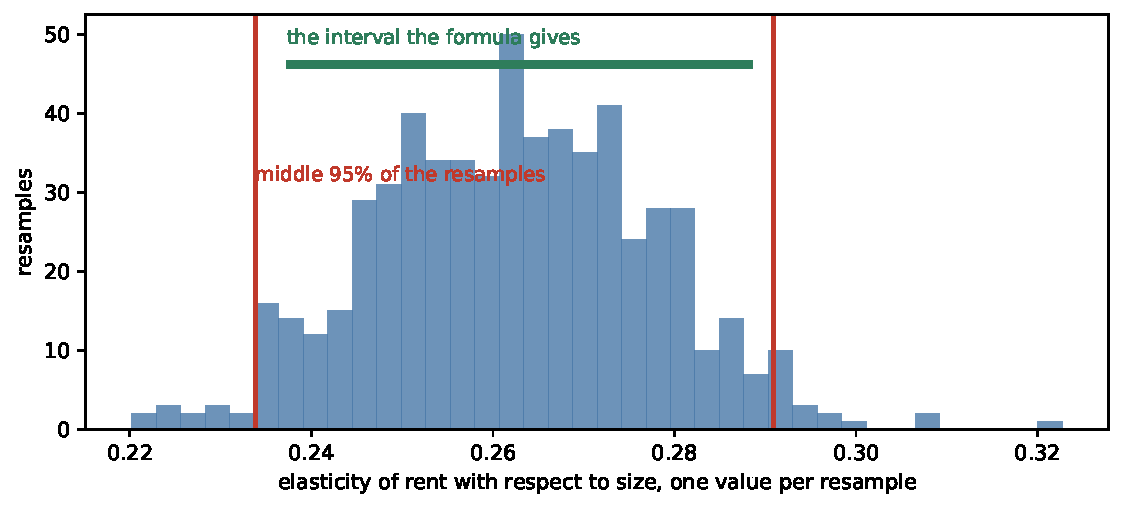
\includegraphics[width=0.84\textwidth]{fig_u6_bootstrap.pdf}
\vspace{0.1em}
\begin{minipage}{0.94\textwidth}\small
The elasticity of rent with respect to size, computed 600 times on 600 resamples. The formula
gives $[0.237, 0.289]$ and the middle 95\% of the resamples is $[0.234, 0.291]$. Where a formula
exists, resampling reproduces it.
\end{minipage}
\end{frame}

\begin{frame}{Quick check: what the resamples are for}
\begin{quickcheck}{thirty seconds}
A student runs 2,000 resamples, takes the average of the 2,000 answers, and reports that as the
estimate instead of the one computed on the original data.
\vspace{0.2em}

Is that a reasonable thing to do, and what were the 2,000 numbers for?
\end{quickcheck}
\onslide<2->{%
\begin{block}{\textbf{Answer}}
The average of the resamples is close to the original estimate and is not an improvement on it;
resampling adds no information that was not already in the sample. The 2,000 numbers are there
for their \emph{spread}, which is what you had no other way of getting. Report the estimate from
the data and the interval from the resamples.
\end{block}}
\end{frame}

% ======================================================================
\section{Intervals with no formula}
% ======================================================================
\begin{frame}{A gap between two medians}
\begin{itemize}
  \item Median rent in Mumbai is Rs 52,000. In Delhi it is Rs 17,000. The gap is
        \textbf{Rs 35,000}.
  \item There is no standard error formula for a difference of medians in any textbook you are
        likely to open.
  \item Resample the Mumbai listings and the Delhi listings separately, take the gap each time,
        and read off the percentiles: \textbf{Rs 32,000 to Rs 39,000}.
\end{itemize}
\begin{practice}{the reporting sentence}
``Mumbai's median rent runs about Rs 35,000 above Delhi's, and the data pins that gap down to
somewhere between Rs 32,000 and Rs 39,000.''
\end{practice}
\end{frame}

\begin{frame}{An interval on an importance score}
\centering
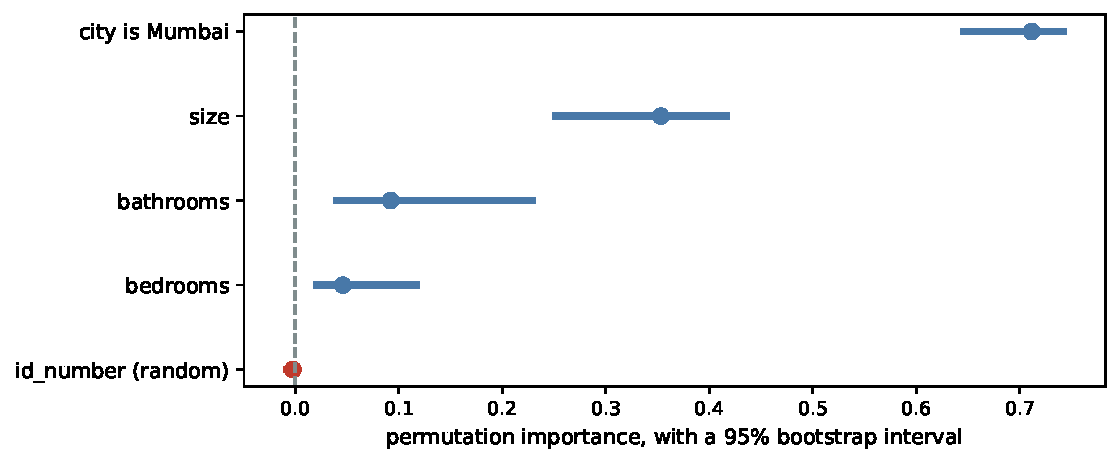
\includegraphics[width=0.84\textwidth]{fig_u6_importance_ci.pdf}
\vspace{0.1em}
\begin{minipage}{0.94\textwidth}\small
The same permutation importances, each with a 95\% bootstrap interval. Four columns sit clearly
away from zero. The random one straddles it, which is the answer to the question the ranking
alone could not settle.
\end{minipage}
\end{frame}

\begin{frame}{The one way to get this wrong}
\begin{itemize}
  \item The importance was measured on held-out rows, so the resampling has to leave that split
        alone: resample the \textbf{training rows only} and score against a test set that was
        never resampled.
  \item Resample first and split afterwards, and the same listing lands in both halves. The forest
        has seen the test rows, shuffling any column then hurts it, and
        \textbf{every} column scores as important, the random one included.
\end{itemize}
\begin{trap}{it fails quietly and in the flattering direction}
Nothing errors. The intervals come back narrow and entirely above zero, and the random column
looks like a finding.
\end{trap}
\end{frame}

\begin{frame}{What to resample, case by case}
\begin{center}\footnotesize
\begin{tabular}{L{0.33\textwidth} L{0.55\textwidth}}
\toprule
\textbf{What you are estimating} & \textbf{What one resample is} \\
\midrule
a mean, a median, a percentile & the rows \\
a gap between two groups & each group separately, each keeping its own size \\
a regression coefficient & the rows, then refit the whole model \\
anything scored on held-out rows & the training rows only, test set untouched \\
whether model A beats model B & the rows, then refit \emph{both} and keep the difference \\
rows that come in clusters & the clusters, not the rows inside them \\
\bottomrule
\end{tabular}
\end{center}
\vspace{0.2em}
\begin{principle}{the rule underneath the table}
Resample whatever you would have had to collect again. If a second sample would have meant 4,743
new listings, resample listings. If it would have meant 60 new buildings, resample buildings.
\end{principle}
\end{frame}

\begin{frame}{Your turn \#1}
\begin{yourturn}{what would you resample?}
For each one, say what a single resample consists of and what you compute on it:
\vspace{0.3em}
\begin{enumerate}\small
  \item The 90th percentile of repair times, with an interval.
  \item The difference in median salary between two departments.
  \item Whether a forest's accuracy is really better than a regression's on the same data.
\end{enumerate}
\end{yourturn}
\end{frame}

\begin{frame}{Your turn \#1: answer}
\begin{itemize}\small
  \item \textbf{(1)} Resample the repair times with replacement, take the 90th percentile of each
        resample, read the percentiles of those.
  \item \textbf{(2)} Resample each department separately, take the gap in medians each time. Keep
        the two groups separate so each keeps its own sample size.
  \item \textbf{(3)} Resample the rows, refit \emph{both} models on each resample, and keep the
        difference in held-out error. If the interval for the difference covers zero, the data
        does not establish that one is better. Refitting both on the same resample is the part
        people skip.
\end{itemize}
\end{frame}

% ======================================================================
\section{Limits}
% ======================================================================
\begin{frame}{What resampling cannot repair}
\begin{itemize}
  \item \textbf{A biased sample.} If the listings over-represent agents, every resample
        over-represents agents too. The interval will be tight around the wrong number.
  \item \textbf{Rows that are not independent.} Several listings from one building are not several
        pieces of evidence. Resample rows and the interval comes out too narrow.
  \item \textbf{A very small sample.} With 12 rows there are only so many distinct resamples, and
        the tails are guesswork.
\end{itemize}
\begin{principle}{what it does and does not do}
Resampling estimates how much your answer moves from sample to sample. It knows nothing about
whether the sample was the right one to take.
\end{principle}
\end{frame}

\begin{frame}{Two things a forest gives you free}
\begin{itemize}
  \item \textbf{Out-of-bag error.} Each tree is fitted on its own bootstrap resample, so about a
        third of the rows are left out of each tree. Score every row using only the trees that did
        not see it and you have a held-out estimate without holding anything out. Here OOB says
        $R^2 = 0.781$ and a real test set says $0.771$.
  \item \textbf{A partial dependence curve.} Sweep one column across its range, holding the others
        as they are, and plot what the forest predicts. It gives a shape rather than a
        coefficient, and it is the closest a forest comes to answering ``how much''.
\end{itemize}
\end{frame}

\begin{frame}{Saying it out loud}
The same finding, three ways. Only the last is usable.
\begin{center}\small
\begin{tabular}{L{0.16\textwidth} L{0.72\textwidth}}
\toprule
\textbf{Too raw} & ``Permutation importance for Mumbai was 0.699 with a bootstrap CI of
$[0.643, 0.745]$.'' \\
\midrule
\textbf{Too loose} & ``The model says location is the big one.'' \\
\midrule
\textbf{Right} & ``Of everything we recorded, whether the flat is in Mumbai is what the model
leans on hardest, and resampling 40 times never changed that. Size is second. The random id we
added as a check came out at zero, which is how we know the ranking is worth reading. None of
this says how much rent goes up, only what the model uses.'' \\
\bottomrule
\end{tabular}
\end{center}
\begin{practice}{the four parts}
What it leaned on, how steady that was, what the noise column did, and the line saying this is
not an effect size.
\end{practice}
\end{frame}

% ======================================================================
\section{Consolidate}
% ======================================================================
\begin{frame}{What to do when the model has no formula}
\small
\begin{enumerate}
  \item \textbf{Want to know which columns the model used?} Permutation importance, not the
        default.
  \item \textbf{Add a column of noise} and check it lands at zero.
  \item \textbf{Want an interval on anything at all?} Resample with replacement, recompute,
        take percentiles.
  \item \textbf{Resample whatever the quantity was computed from}, and leave any train/test split
        where it is.
  \item \textbf{Want an honest error for a forest?} Out-of-bag, or a test set.
  \item \textbf{Report the estimate from the data} and the interval from the resamples.
  \item \textbf{Say what the interval does not cover:} bias, dependence, and whether the sample
        was the right one.
\end{enumerate}
\end{frame}

\begin{frame}{The traps}
\begin{trap}{the ones that bite most often}
\begin{itemize}
  \item Reading an importance ranking as a ranking of effect sizes.
  \item Reporting the default importance on data with an id, a timestamp, or any column with many
        distinct values.
  \item Reading an importance score as having units or a direction.
  \item Resampling without replacement, which produces no spread at all.
  \item Resampling before a train/test split, so the same row lands on both sides.
  \item Quoting a bootstrap interval as though it covered sampling bias.
  \item Averaging the resamples and reporting that as the estimate.
\end{itemize}
\end{trap}
\end{frame}

\begin{frame}{What you should be able to do with software}
\small
\begin{center}\footnotesize
\begin{tabular}{p{0.44\textwidth} p{0.46\textwidth}}
\toprule
\textbf{You should be able to} & \textbf{What you would reach for} \\
\midrule
Fit a forest and get its held-out error &
\texttt{RandomForestRegressor(oob\_score=True)} \\
Get the default importance & \texttt{forest.feature\_importances\_} \\
Get permutation importance & \texttt{permutation\_importance(forest, X\_test, y\_test)} \\
Draw one resample & \texttt{df.sample(len(df), replace=True)} \\
Turn resamples into an interval & \texttt{np.percentile(boot, [2.5, 97.5])} \\
Check an importance method & add a random column and refit \\
\bottomrule
\end{tabular}
\end{center}
\end{frame}

\begin{frame}{Where we go next}
\begin{itemize}
  \item Every interval so far has come from one of two places: a formula that assumed a
        distribution, or resampling that assumed almost nothing.
  \item \textbf{Unit 7} starts on where the formulas come from: probability, and what chance alone
        produces.
  \item The bootstrap returns there with a reason attached, rather than as a recipe that happens
        to work.
\end{itemize}
\end{frame}

\end{document}
